\chapter{Activity Flow glyphs}

%[Note on the color code:
%\textcolor{blue}{The glyphs that have been thoroughly discussed, and are considered frozen, are represented in blue}.
%\textcolor{green}{The glyphs that have been thoroughly discussed, but are still posing problems are represented in green}.
%\textcolor{red}{The glyphs that have been proposed but for which in-depth discussion is yet to come are represented in red}.]

This chapter provides a catalog of the graphical symbols available for representing entities in \AFs. In \chap{af:grammar} beginning on page~\pageref{chp:af:grammar}, we describe the rules for combining these glyphs into a legal SBGN \AF, and in \chap{af:layout} beginning on page~\pageref{chp:af:layout}, we describe requirements and guidelines for the way that \AFms are visually organized.

\section{Overview}


To set the stage for what follows in this chapter, we first give a brief overview of some of the concepts in the \AF notation with the help of an example shown in \fig{af:1}.

The diagram illustrates the regulation of peroxisome proliferator-activated receptor delta (PPAR delta, a nuclear hormone receptor) on brown fat metabolism, a redraw from Fig 7E of Pan et. al~\cite{Pan:2009}.  The rectangle nodes represent \emph{biological activities} - activities from biological materials.  The type of material is indicated in the units of information decorating on the activity nodes (See \sect{af:biologicalActivity}).  Each biological activity can influence, or be influenced by, other biological activities, and such relationships are represented in \AF by lines with arrows and other decorations.  It should be noted that the essence of \AF is to show the flow of activities from one entity to another or within the same entity.  For example, in the diagram, it shows that PPAR$\delta$ positively influences the Twist-1 gene expression.  The underlying mechanisms of how the influence occurs may not be known and is not captured in the diagram.  If the mechanism is known, the details should be described in a \PD and/or \ER map.

\tab{component-summary} summarizes the different SBGN abstractions described in this chapter.

\newcolumntype{P}[1]{>{\raggedright\hspace{0pt}\arraybackslash}p{#1}}

\begin{table}[bh]
  \centering
  \small
  \begin{tabular}{@{}llP{2.4in}P{1.6in}@{}}
    \toprule
    \textbf{Component} & \textbf{Abbrev.} & \textbf{Role} & \textbf{Examples}\\
    \midrule
    Activity node
    & AN
    & A functional unit that can affect, or be affected by, another functional unit
    & Biological activity \\[0.5em]

    Container node	
    & CN
    & An encapsulation of one or more other SBGN constructs
    & Compartments \\[1.6em]

    Modulating arc
    & MA
    & Links between different activities to indicate influences
    & Positive influence, Negative influence \\[0.5em]
    
    Auxiliary units
    & AU
    & A decorating glyph to the AN to provide additional information of the node, such as the property where the activity is originated
    & Unit of information   \\[1.6em]
    
    Logical operators
    & ---
    & Combines one or several inputs into one output
    & Boolean \emph{and}, \emph{or}, \emph{not}, \emph{delay} \\
    \bottomrule
  \end{tabular}
  \caption{Summary of \AF components and their roles.}
  \label{tab:component-summary}
\end{table}

\begin{figure}[H]
\centering
\vspace*{-0.75em}
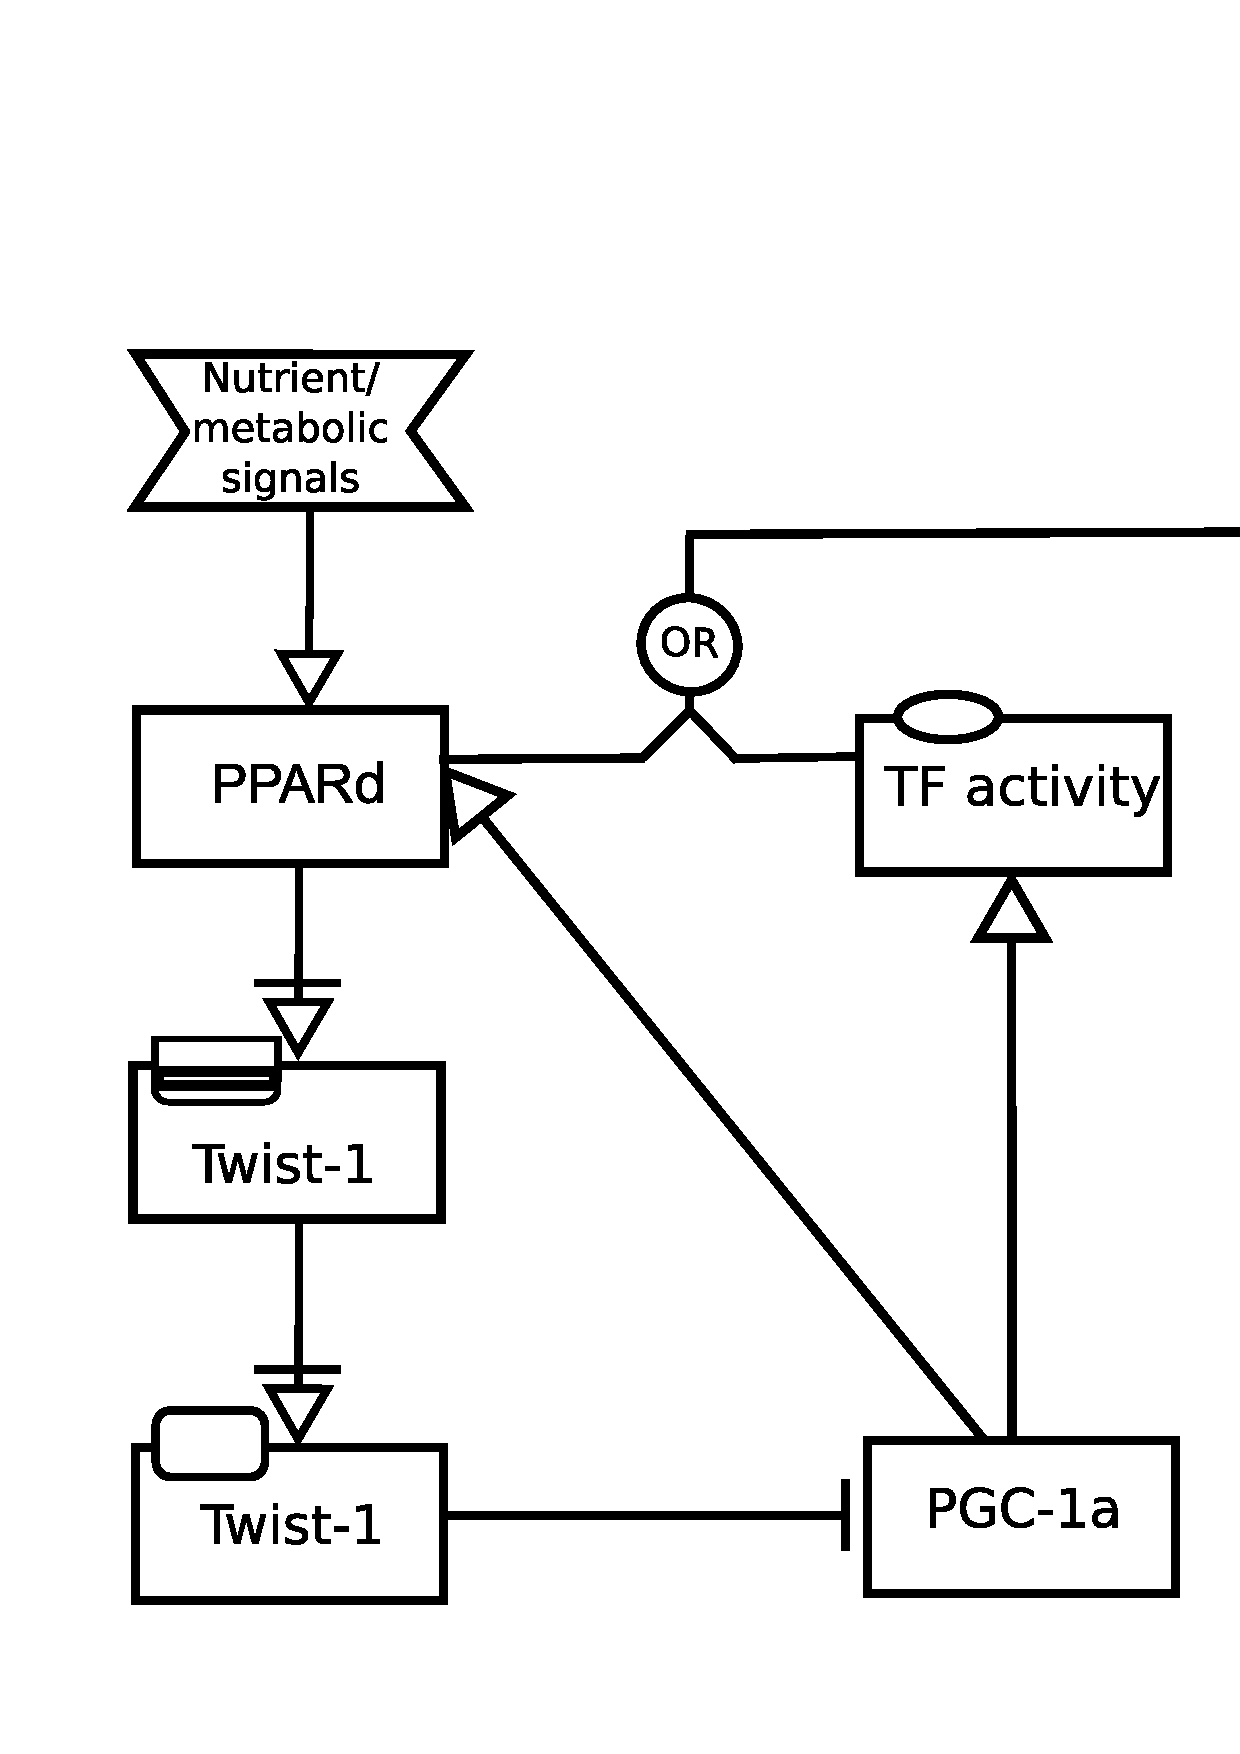
\includegraphics[scale=0.4]{examples/PPAR}
\caption{This example of \AF is based on Figure 7E of Pan el. al.~\cite{Pan:2009}.  It depicts the effect of nutrients and metabolic signals on brown fat metabolism through PPAR$\delta$. The signal, shown as a perturbation, positively influences the nuclear hormone receptor PPAR$\delta$, which in turn stimulates the Twist 1 gene expression.  Please note the different \emph{units of information} on Twist-1 activity nodes that indicate the activity from different biological materials (gene and protein). The Twist-1 protein negatively influences the PGC-1$\alpha$ activity, which positively influences PPAR$\delta$ and other unspecified transcription factor activity to stimulate the expression of genes for brown fat energy dissipation. Therefore, the Twist-1, induced by PPAR$\delta$, serves as a negative feedback regulator of PGC-1$\alpha$ in brown fat metabolism.}
\label{fig:af:1}
\end{figure}


\section{Controlled vocabularies used in \SBGNAFLone}\label{af:sec:CVs}

%%%%%%%%%%%%%%%%%%%%%%%%%%%%%%%%%%%%%%%%%%%%%%%%%%%%%%%%%%%%%%%%%%%%%%
%%%%                   Controlled vocabularies
%%%%%%%%%%%%%%%%%%%%%%%%%%%%%%%%%%%%%%%%%%%%%%%%%%%%%%%%%%%%%%%%%%%%%%

\color{red}
What controlled vocabulary should we use? SBO? GO molecular function?
\normalcolor

Some glyphs in SBGN \AF can contain particular kinds of textual annotations conveying information relevant to the purpose of the glyph.  These annotations are \glyph{units of information} (\sect{af:unitInfo}).  An example is in the case of a compartment, which can have a unit of information conveying physical characteristics of the compartment .

The text that appears as the unit of information decorating an Activity Node (AN) od Container Node (CN) must in most cases be prefixed with a controlled vocabulary term indicating the type of information being expressed. Without the use of controlled vocabulary prefixes, it would be necessary to have different glyphs to indicate different classes of information; this would lead to an explosion in the number of symbols needed. 

In the rest of this section, we describe the controlled vocabularies (CVs) used in \SBGNAFLone. Some CV terms are predefined by SBGN, but unless otherwise noted, they are not the only terms permitted. Authors may use other CV values not listed here, but in such cases, they should explain the term's meanings in a Figure legend or other text accompanying the map.

\subsection{Activity node material types}
\label{sec:af:material-types-cv}

The material type of an AFN indicates its chemical structure.  A list of common material types is shown in \tab{af:material-types-cv}, but others are possible.  The values are to be taken from the \sbo (\sbourl), specifically from the branch having identifier \sboid{SBO:0000240} ($\!$\emph{material entity} under \emph{participant}$\rightarrow$\emph{physical participant}).  The labels are defined by \SBGNAFLone.

\begin{table}[h]
  \centering
  \begin{tabular}{l>{\ttfamily}l>{\ttfamily}l}
    \toprule
    \textbf{Name}              & \textbf{\rmfamily Label} & \textbf{\rmfamily SBO term} \\
    \midrule
    Non-macromolecular ion     & mt:ion  & SBO:0000327\\
    Non-macromolecular radical & mt:rad  & SBO:0000328\\
    Ribonucleic acid           & mt:rna  & SBO:0000250\\
    Deoxribonucleic acid       & mt:dna  & SBO:0000251\\
    Protein                    & mt:prot & SBO:0000297\\
    Polysaccharide             & mt:psac & SBO:0000249\\
    \bottomrule
  \end{tabular}
  \caption{A sample of values from the \emph{material types} controlled
    vocabulary (\sect{af:material-types-cv}).}
  \label{tab:af:material-types-cv}
\end{table}

The material types are in contrast to the \emph{conceptual types} (see below).  The distinction is that material types are about physical composition, while conceptual types are about roles.  For example, a strand of RNA is a physical artifact, but its use as messenger RNA is a role.

\subsection{Activity node conceptual types}
\label{sec:af:conceptual-types-cv}

An AFN's \emph{conceptual type} indicates its function within the context of a given \AF.  A list of common conceptual types is shown in \tab{af:conceptual-types-cv}, but others are possible.  The values are to be taken from the \sbo (\sbourl), specifically from the branch having identifier \sboid{SBO:0000241} ($\!$\emph{conceptual entity} under \emph{participant}$\rightarrow$\emph{physical participant}).  The labels are defined by \SBGNAFLone.

\begin{table}[h]
  \centering
  \begin{tabular}{l>{\ttfamily}l>{\ttfamily}l}
    \toprule
    \textbf{Name}              & \textbf{\rmfamily Label} & \textbf{\rmfamily SBO term} \\
    \midrule
    Gene                      & ct:gene   & SBO:0000243\\
    Transcription start site  & ct:tss    & SBO:0000329\\
    Gene coding region        & ct:coding & SBO:0000335\\
    Gene regulatory region    & ct:grr    & SBO:0000369\\
    Messenger RNA             & ct:mRNA   & SBO:0000278\\
    \bottomrule
  \end{tabular}
  \caption{A sample of values from the \emph{conceptual types} vocabulary
    (\sect{af:conceptual-types-cv}).}
  \label{tab:af:conceptual-types-cv}
\end{table}

\subsection{Physical characteristics of compartments}
\label{sec:af:physical-characteristics-cv}

\SBGNAFLone defines a special unit of information for describing certain common physical characteristics of compartments.  \tab{af:physical-characteristics-cv} lists the particular values defined by \SBGNAFLone.  The values correspond to the \sbo branch with identifier \sboid{SBO:0000255} (\emph{physical characteristic} under \emph{quantitative parameter}).

\begin{table}[h]
  \centering
  \begin{tabular}{l>{\ttfamily}l>{\ttfamily}l}
    \toprule
    \textbf{Name}   & \textbf{\rmfamily Label} & \textbf{\rmfamily SBO term} \\
    \midrule
    Temperature   & pc:T  & SBO:0000147\\
    Voltage       & pc:V  & SBO:0000259\\
    pH            & pc:pH & SBO:0000304\\
    \bottomrule
  \end{tabular}
  \caption{A sample of values from the \emph{physical
      characteristics} vocabulary (\sect{af:physical-characteristics-cv}).}
  \label{tab:af:physical-characteristics-cv}
\end{table}

%\subsection{Cardinality}
%\label{sec:af:cardinality-cv}
%
%\SBGNAFLone defines a special unit of information usable on multimers for describing the number of monomers composing the multimer.  \tab{af:cardinality-cv} shows the way in which the values must be written.  Note that the value is a unitary number, and not (for example) a range.  There is no provision in \SBGNAFLone for specifying a range in this context because it leads to problems of entity identifiability.
%
%\begin{table}[h]
%  \centering
%  \begin{tabular}{l>{\ttfamily}l>{\ttfamily}l}
%    \toprule
%    \textbf{Name}   & \textbf{\rmfamily Label} & \textbf{\rmfamily SBO term} \\
%    \midrule
%    cardinality    & N:\#  & SBO:0000364\\
%    \bottomrule
%  \end{tabular}
%  \caption{The format of the possible values for the
%    \emph{cardinality} unit of information
%    (\sect{af:cardinality-cv}).  Here, \texttt{\#} stands for the
%    number; for example, ``\texttt{N:5}''.}
%  \label{tab:af:cardinality-cv}
%\end{table}


%%%%%%%%%%%%%%%%%%%%%%%%%%%%%%%%%%%%%%%%%%%%%%%%%%%%%%%%%%%%%%%%%%%%%%
%%%%                   Activity nodes
%%%%%%%%%%%%%%%%%%%%%%%%%%%%%%%%%%%%%%%%%%%%%%%%%%%%%%%%%%%%%%%%%%%%%%

\section{Activity nodes}\label{sec:af:ANs}

An Activity Node (AN) represents the activity of an entity or an entity pool, but not the entities themselves. For instance, multiple activity nodes can be used to represent different activities of a particular entity, while one activity node can be used to represent the activity of a complex multimer. In addition to activities of material entities, \SBGNAFLone represents activity from two conceptual entities: \emph{perturbation}, \emph{phenotype}.  Auxiliary units such as state variables are not shown on the activity nodes.  Each activity is displayed only once in one compartment.


\subsection{Glyph: \glyph{Biological activity}}
\label{sec:af:biologicalActivity}


\SBGNAFLone uses one glyph to represent activities from all biological entities, collectively they are called \emph{biological activity}. The nature of the molecule that the activity comes from, eg., simple chemical or macromolecule, can be encoded in the \emph{units of information} (\sect{af:unitInfo}). 

It should be noted that the \emph{biological activity} is not equivalent to a biological entity per se.  A biological activity can come from one biological entity, a part of an entity, or a combination of  them.  It is up to the users to determine how to represent it in their diagram.  For example, a protein kinase receptor such as an EGF receptor, has two activities, the binding activity that allows the extracellular part of the receptor to bind to the ligand, and the kinase activity that is capable of phosphorylating the downstream protein and initiating the intracellular signaling.  The user can choose to use two nodes to represent each activity, or to use one node to represent the overall "EGF receptor activity". 

\begin{glyphDescription}

\glyphSboTerm SBO:0000412 ! biological activity

\glyphContainer An \glyph{biological activity} is represented by a rectangle, as shown in \fig{af:biologicalActivity}.

\glyphLabel An \glyph{biological activity} is identified by a label placed in an unbordered box containing a string of characters.  The characters can be distributed on several lines to improve readability, although this is not mandatory.  The label box must be attached to the center of the container.  The label may spill outside of the container.

\glyphAux A \glyph{biological activity} can carry a \glyph{unit of information} (\sect{af:unitInfo}), which can provide information such as the nature of the entity from which the activity originated.  Specific glyphs are used to represent different types of entities (\sect{af:unitInfo}).  The center of the bounding box of a \glyph{unit of information} is located on the mid-line of the border of the macromolecule.  The label in the \glyph{unit of information}, which is optional, indicates the name of the molecule where the activity comes from, as shown in \fig{af:EGFR}

\end{glyphDescription}

\begin{figure}[H]
  \centering
  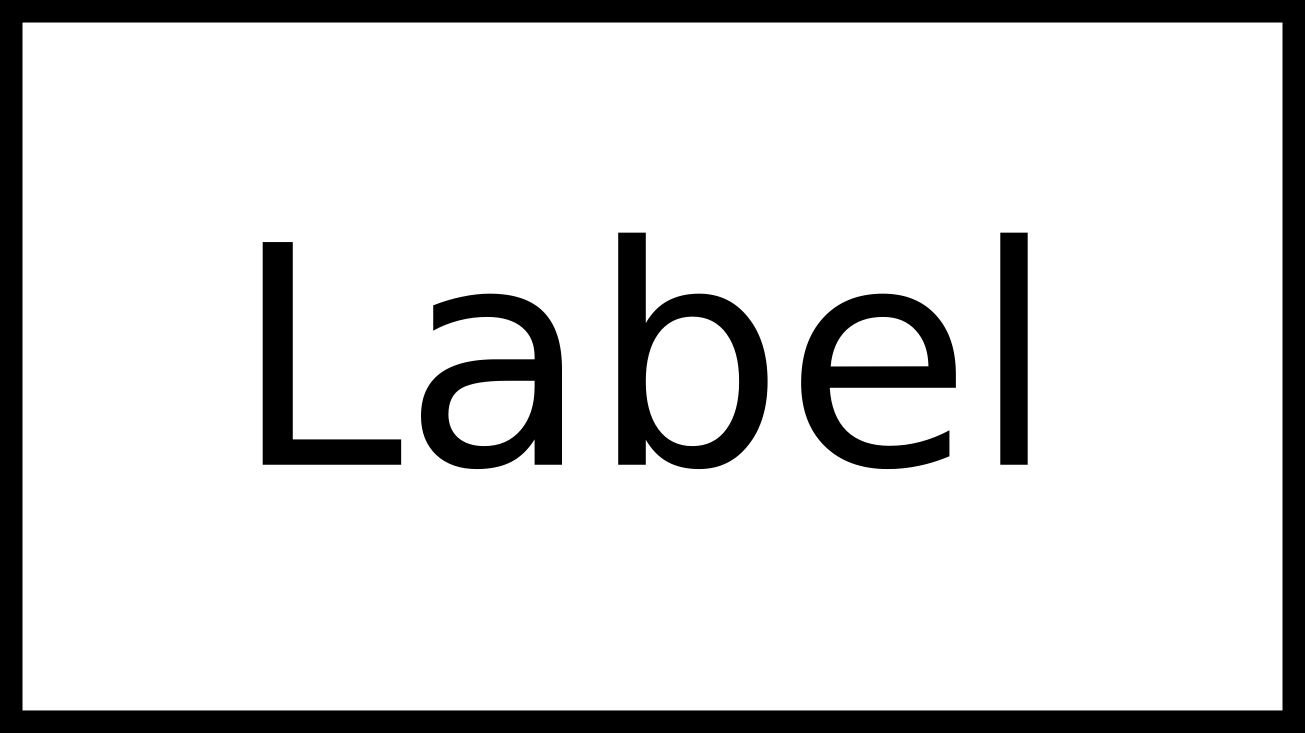
\includegraphics[scale = 0.5]{images/biologicalActivity}
  \caption{The \AF glyph for \glyph{biological activity}.}
  \label{fig:af:biologicalActivity}
\end{figure}

\begin{figure}[H]
  \centering
  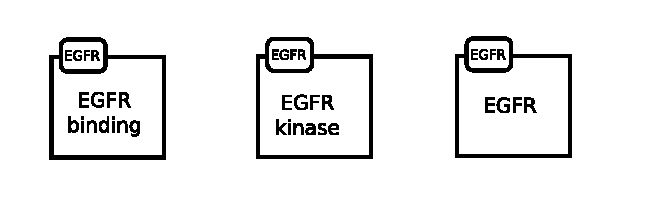
\includegraphics[scale = 1]{examples/EGFR}
  \caption{An example of \AF glyphs of EGFR activities.  Since EGFR protein has both binding and kinase activities, each of those activity can be represented by different nodes, labeled as \emph{EGFR binding} and \emph{EGFR kinase}.  One node can be used to represent the overall activity of \emph{EGFR}.  The label in the \glyph{unit of information} indicates the protein that the activities come from.  In this example, all three activities come from the same EGFR protein}
  \label{fig:af:EGFR}
\end{figure}
\subsection{Glyph: \glyph{Perturbation}}
\label{sec:af:perturbation}

Biochemical networks can be affected by external influences. Those influences can be well-defined physical perturbations, such as a light pulse or a change in temperature; they can also be more complex and not well-defined phenomena, for instance, glucose deprivation, stress. For these situations, SBGN provides the perturbation glyph. 

\begin{glyphDescription}

\glyphSboTerm SBO:0000357 ! perturbation

\glyphContainer A \glyph{perturbation} is represented by a modified hexagon
having two opposite concave faces, as illustrated in \fig{af:perturbation}.

\glyphLabel A \glyph{perturbation} is identified by a label placed in an unbordered box containing a string of characters.  The characters can be distributed on several lines to improve readability, although this is not mandatory.  The label box must be attached to the center of the \glyph{perturbation} container.  The label may spill outside of the container.

\end{glyphDescription}

\begin{figure}[H]
  \centering
  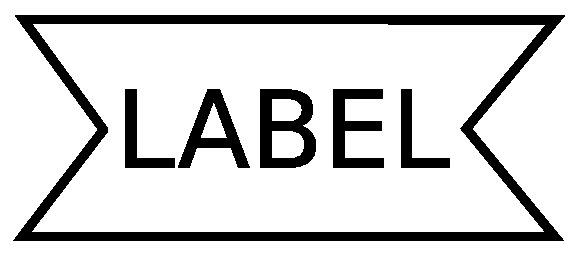
\includegraphics[scale=0.3]{images/perturbation}
  \caption{The \AF glyph for \glyph{perturbation}.}
  \label{fig:af:perturbation}
\end{figure}

\subsection{Glyph: \glyph{Phenotype}}
\label{sec:af:phenotype}

A biochemical network can generate phenotypes or affect biological processes. Such processes can take place at different levels and are independent of the biochemical network itself. To represent these processes in a diagram, SBGN defines the \glyph{phenotype} glyph.

\begin{glyphDescription}

\glyphSboTerm
SBO:0000358 ! phenotype

\glyphContainer A \glyph{phenotype} is represented by an elongated
hexagon, as illustrated in \fig{af:phenotype}.

\glyphLabel An \glyph{phenotype} is identified by a label placed in an
unbordered box containing a string of characters.  The characters can be
distributed on several lines to improve readability, although this is not
mandatory.  The label box must be attached to the center of the
\glyph{phenotype} container.  The label may spill outside of the container.

\end{glyphDescription}

\begin{figure}[H]
  \centering
  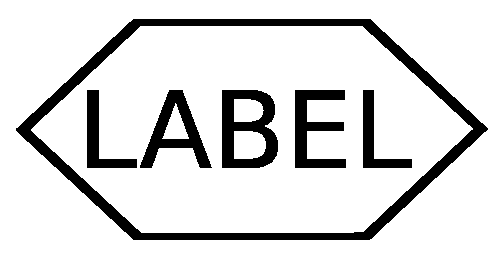
\includegraphics[scale = 0.4]{images/phenotype}
  \caption{The \AF glyph for \glyph{phenotype}.}
  \label{fig:af:phenotype}
\end{figure}


%%%%%%%%%%%%%%%%%%%%%%%%%%%%%%%%%%%%%%%%%%%%%%%%%%%%%%%%%%%%%%%%%%%%%%
%%%%                   Auxiliary units
%%%%%%%%%%%%%%%%%%%%%%%%%%%%%%%%%%%%%%%%%%%%%%%%%%%%%%%%%%%%%%%%%%%%%%

\section{Auxiliary units}\label{sec:af:AUs}

\subsection{Glyph: \glyph{Unit of information for Biological activity}}
\label{sec:af:unitInfo}

When representing biological activities, it is often useful to illustrate the nature of the entity where the activity is originated, eg., whether the activity is from a macromolecule (protein or nucleic acid), or from a chemical compound.  The \SBGNAFLone \glyph{unit of information} is used to add such information to a glyph.  It represents the information in two ways.  First, different symbols are used to represent the nature of the entity where the activity is from, e.g.., macromolecule, nucleic acid feature, or complex.  These symbols are identical to the \glyph{entity pool node} symbols in SBGN \PDl.  Second, names of the entity (gene names, protein names) are usually provided as labels in the \glyph{unit of information} container.

\begin{glyphDescription}

\glyphSboTerm Not applicable.

\glyphContainer A unit of information is represented by containers of different shapes, depending on the nature of the entity where the biological activity is from. There are a total of five types of unit of information, as shown in \fig{af:unitInfo}.   Below is a summary of the five glyphs.

\begin{description}
\item[A.] macromolecule -- Macromolecules are biochemical substances that are built up from the covalent linking of pseudo-identical units. Examples of macromolecules include proteins, nucleic acids (RNA, DNA), and polysaccharides (glycogen, cellulose, starch, etc.).  
A unit of information of a macromolecule is represented by a rectangle with rounded corners, as illustrated in (A) of \fig{af:unitInfo}.  This container is used to decorate a biological activity that is originated from a macromolecule, such as a protein, a nucleic acid, or a complex sugar.

\item[B.] nucleic acid feature -- The Nucleic acid feature construct in SBGN is meant to represent a fragment of a macromolecule carrying genetic information. A unit of information of a nucleic acid feature is represented by a rectangle whose bottom half has rounded corners, as shown in (B) of  \fig{af:unitInfo}.

\item[C.] simple chemical -- A simple chemical is a chemical compound that is not formed by the covalent linking of pseudo-identical residues. Examples of simple chemicals are an atom, a monoatomic ion, a salt, a radical, a solid metal, a crystal, etc. 
A unit of information of a simple chemical is represented by a circular container, as shown in (C) of \fig{af:unitInfo}.

\item[D.] unspecified entity -- An unspecified entity is used to represent the entity type that is unknown or simply not relevant to the purposes of the map. This arises, for example, when the existence of the entity has been inferred indirectly, or when the entity is merely a construct introduced for the needs of a map, without direct biological relevance. A unit of information of an unspecified entity is represented by an elliptic container, as shown in (D) of \fig{af:unitInfo}.  It is used to decorate a biological activity that is originated from an unspecified entity.

\item[E.] complex -- A complex represents a biochemical entity composed of other biochemical entities, whether macromolecules, simple chemicals, or other complexes. The resulting entity may 
have its own identity, properties and function in an SBGN map. A unit of information of a complex is represented by an octagon as shown in (E) of \fig{af:unitInfo}.  It is used to decorate a biological activity that is originated from a complex.

\item[F.] perturbation -- Biochemical networks can be affected by external influences. Those influences can be well-defined physical perturbations, such as a light pulse or a change in temperature; they can also be more complex and not well-defined phenomena, for instance, glucose deprivation, stress.  A unit of information of a perturbation is represented by a modified hexagon
having two opposite concave faces, as illustrated in F of  \fig{af:unitInfo}.  It is used to decorate a biological activity when it is originated from a perturbation.
\end{description}

\begin{figure}[H]
  \centering
  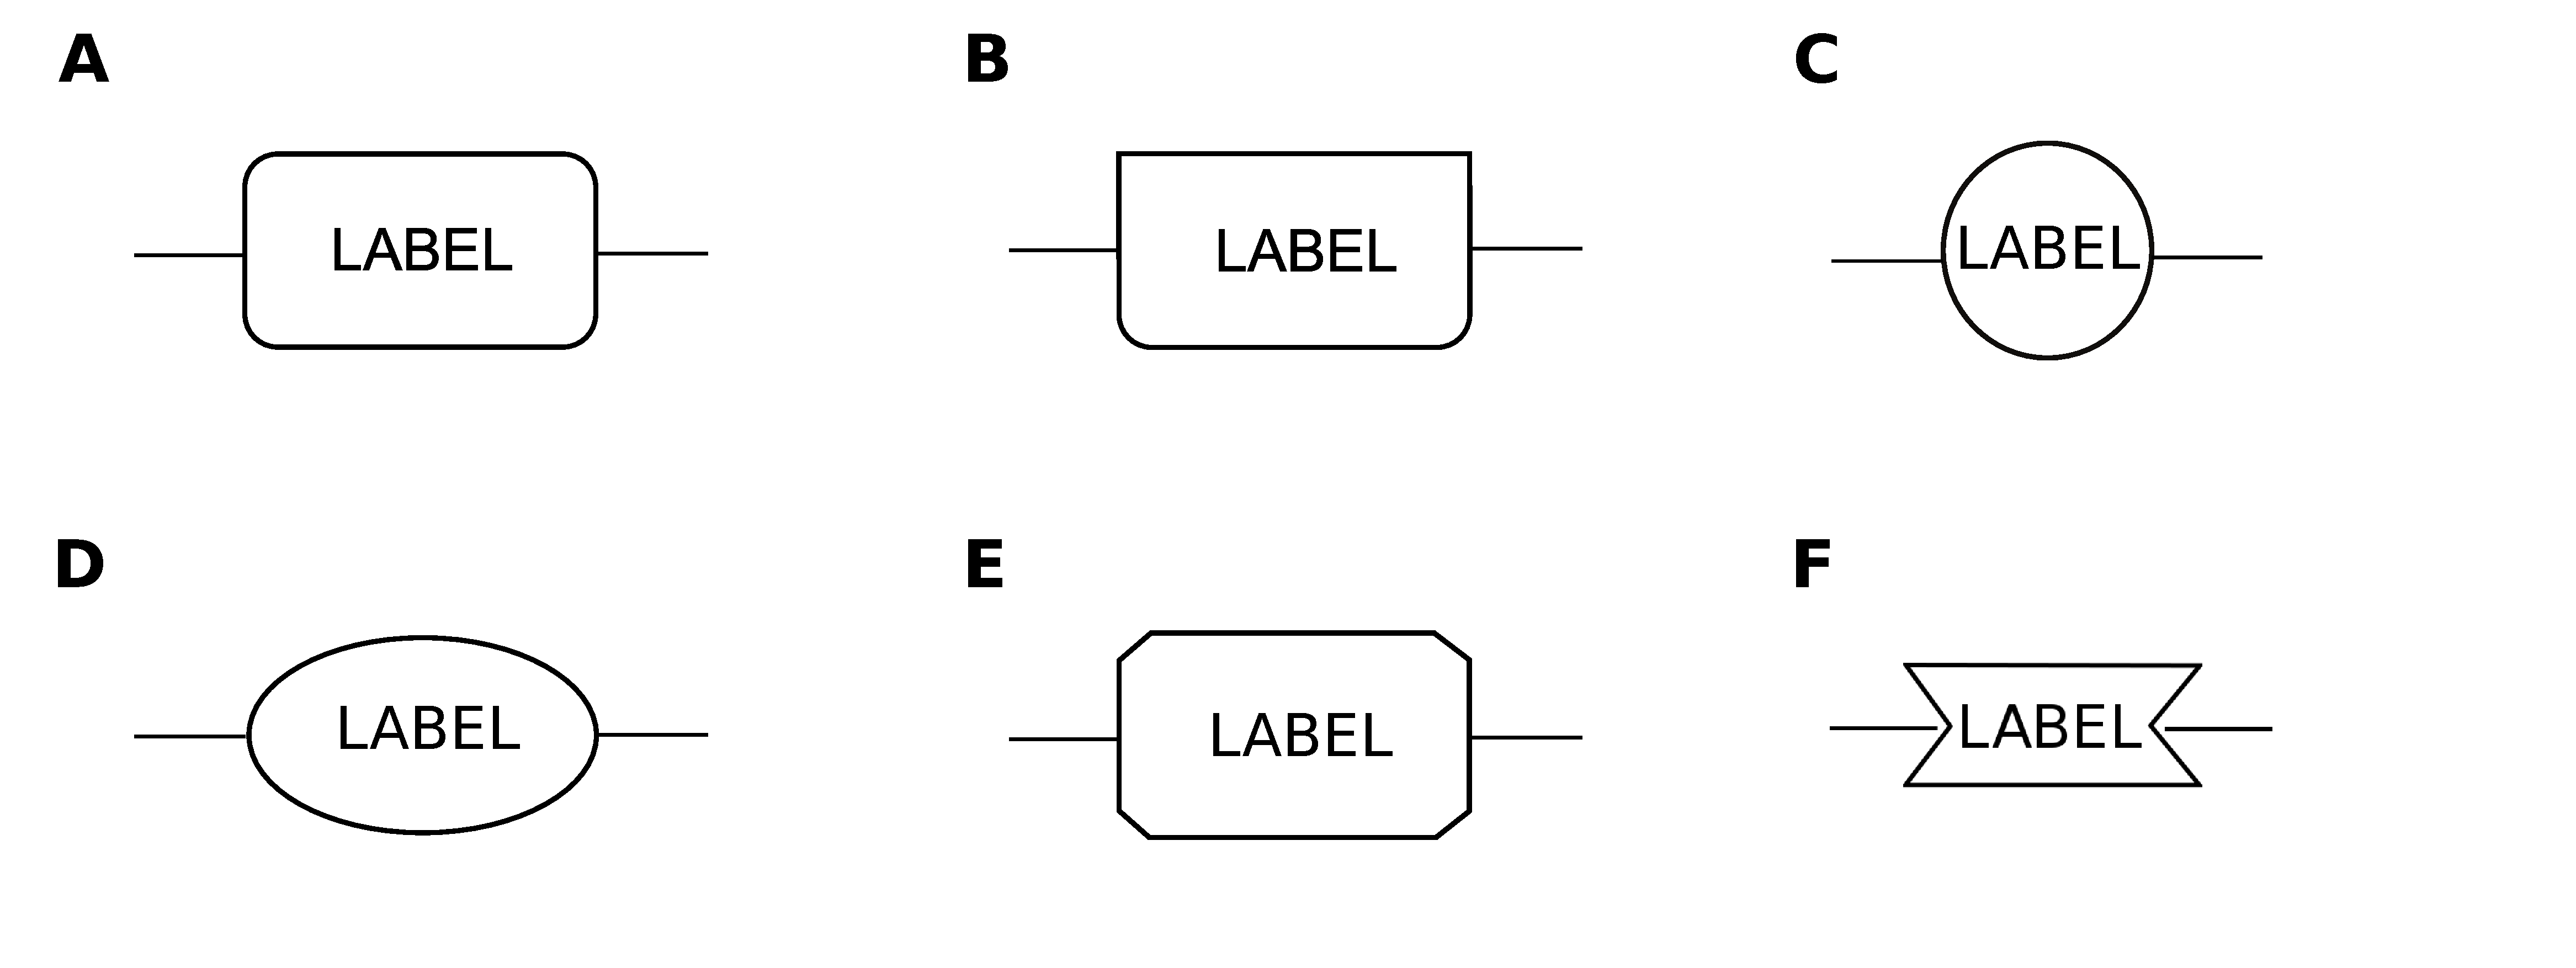
\includegraphics[scale = 0.2]{images/unitInformation_ba}
  \caption{The \AF glyph for \glyph{unit of information}.}
  \label{fig:af:unitInfo}
\end{figure}

\begin{figure}[H]
  \centering
  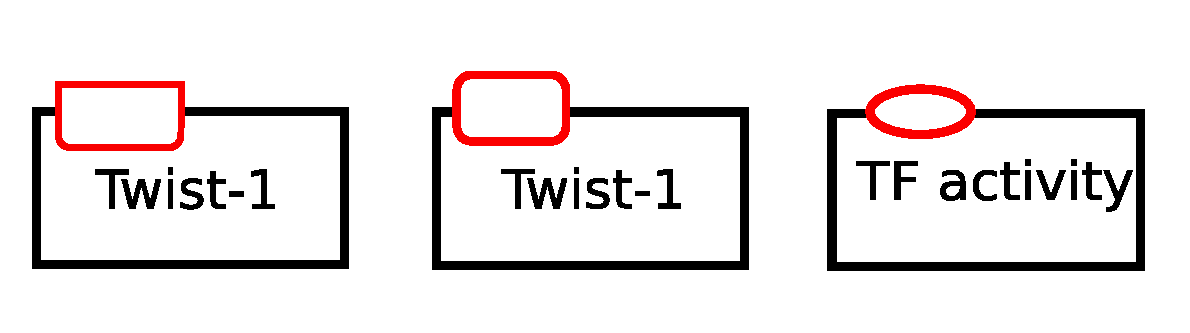
\includegraphics[scale = 0.5]{examples/unitofinformation}
  \caption{Examples of \glyph{unit of information} used on \glyph{biological activity node} to indicate that the \emph{Twist-1 activity} is from a \emph{nucleic acid feature} or a \emph{macromolecule}, or a \emph{transcription factor activity} from an \emph{unspecified} entity.}
  \label{fig:af:unitofinfo}
\end{figure}

\fig{af:unitofinfo} shows examples taken from \fig{af:1}, where \emph{units of information} is used on Activity Nodes to illustrate the properties of the entities that the activities are originated from.

The long side of the glyphs above (except for simple chemical) should be oriented parallel to the border of the \glyph{AN} being annotated by the \glyph{unit of information}. The center of the bounding box of a \glyph{state of information} should be located on the mid-line of the border of the \glyph{AN}.

\glyphLabel A \glyph{unit of information} is not required to carry any label.   If a label is desired, it should be placed in an unbordered box containing a string of characters. The characters can be distributed on several lines to improve readability, although this is not mandatory.  The label box must be attached to the center of the container. The label may spill outside of the container.  The label defines the information carried by the \glyph{unit of information}.

\glyphAux A \glyph{unit of information} does not carry any auxiliary items.

\end{glyphDescription}

\subsection{Glyph: \glyph{Unit of information for Compartment}}
\label{sec:af:unitInfoComp}

A \emph{unit of information} can be used to decorate a compartment to convey information about physical characteristics of the compartments (\sect{af:physical-characteristics-cv}). 

\begin{glyphDescription}

\glyphSboTerm Not applicable.

\glyphContainer A \emph{unit of information} for compartment is represented by a rectangle as shown in \fig{compunitInfo}.  The long side of the rectangle should be oriented parallel to the border of the \glyph{compartment} being annotated by the \glyph{unit of information}. The center of the bounding box of a \glyph{state of information} should be located on the mid-line of the border of the \glyph{compartment}.

\begin{figure}[H]
  \centering
  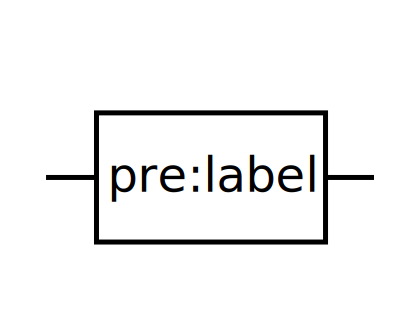
\includegraphics[scale = 0.5]{images/unitInformation}
  \caption{The \AF glyph for \glyph{unit of information}.}
  \label{fig:compunitInfo}
\end{figure}

\glyphLabel A \glyph{unit of information} is identified by a label placed in an unbordered box containing a string of characters.  The characters can be distributed on several lines to improve readability, although this is not mandatory.  The label box must be attached to the center of the container.  The label may spill outside of the container.

The label defines the information carried by the \glyph{unit of information}.  For certain predefined types of information for the compartment, such as physical characteristics, SBGN defines specific prefixes that must be included in the label to indicate the type of information in question.  The controlled vocabularies predefined in \SBGNAFLone are described in \sect{af:physical-characteristics-cv} and summarized in the following list:

\begin{center}
  \begin{itemize}\setlength{\parskip}{0ex}
  \item{pc:T} Temperature (SBO:0000147)
  \item{pc:V} Voltage (SBO:0000259)
  \item{pc:pH} pH (SBO:0000304)
  \end{itemize}
\end{center}

    
\glyphAux A \glyph{unit of information} does not carry any auxiliary items.  

\end{glyphDescription}




%%%%%%%%%%%%%%%%%%%%%%%%%%%%%%%%%%%%%%%%%%%%%%%%%%%%%%%%%%%%%%%%%%%%%%
%%%%                   Container nodes
%%%%%%%%%%%%%%%%%%%%%%%%%%%%%%%%%%%%%%%%%%%%%%%%%%%%%%%%%%%%%%%%%%%%%%

\section{Container nodes}
\label{sec:af:CNs}

\glyph{Containers} are SBGN constructions that contain one or several other SBGN constructs.  In \SBGNAFLone \glyph{compartment} and \glyph{submap} are the only container nodes.

\subsection{Glyph: \glyph{Compartment}}\label{sec:compartment}

In order to describe biochemical and cellular events, it is useful to define the notion of pools. A pool is an ensemble of participants that  can be considered to be identical for the events in which they are involved. A compartment is a logical or physical structure that contains pools. A pool can only belong to one compartment. Therefore, the ``same'' biochemical species located in two different compartments are in fact two different pools.

\begin{glyphDescription}

\glyphSboTerm  SBO:0000289 ! functional compartment

\glyphContainer A compartment is represented by a surface enclosed in a continuous border or located between continuous borders. These borders should be noticeably thicker than the borders of the ANs. A compartment can take \textbf{any} geometry. A compartment must always be entirely enclosed.

\glyphLabel The identification of the compartment is carried by an unbordered box containing a string of characters. The characters can be distributed on several lines to improve readability, although this is not mandatory. The label box can be attached anywhere in the container box. Note that the label can spill-over from the container box.

\glyphAux A \glyph{compartment} can carry a certain number of \glyph{units of information}, that will add information for instance about the physical environment, such as pH, temperature or voltage, see \sect{af:unitInfo}.  The center of the bounding box of a \glyph{unit of information} is located on the mid-line of the border of the compartment.

\end{glyphDescription}

\begin{figure}[H]
  \centering
  \includegraphics[scale = 0.3]{images/compartment}
  \caption{The \AF glyph for \glyph{compartment}.}
  \label{fig:af:compartment}
\end{figure}



\section{Glyph: \glyph{Submap}}
\label{sec:submap}

A \glyph{submap} is used to encapsulate processes (including all types of nodes and edges) within one glyph.  The submap hides its content to the users, and displays only input terminals (or ports), linked to \glyph{ANs}. In the case of an SBGN diagram that is made available through a software tool, the content of a submap may be available to the tool.  A user could then ask the tool to expand the submap, for instance by clicking on the icon for the submap.  The tool might then expand and show the submap within the same diagram (on the same canvas), or it might open it in a different canvas.

\begin{glyphDescription}

\glyphSboTerm SBO:0000395 ! encapsulating process

\glyphContainer The \glyph{submap} is represented as a rectangle box to remind the viewer that it is fundamentally a biological activity node.

\glyphLabel The identification of the \glyph{submap} is carried by an unbordered box containing a string of characters.  The characters may be distributed on several lines to improve readability, although this is not mandatory.  The label box has to be attached to the center of the container box.

\glyphAux A \glyph{submap} carries labeled terminals.  When the submap is represented folded, those terminals are linked to external \glyph{ANs}.  In the unfolded view, exposing the internal structure of the submap, a set of \glyph{tags} point to the corresponding internal \glyph{ANs}.

\end{glyphDescription}

\begin{figure}[H]
  \centering
  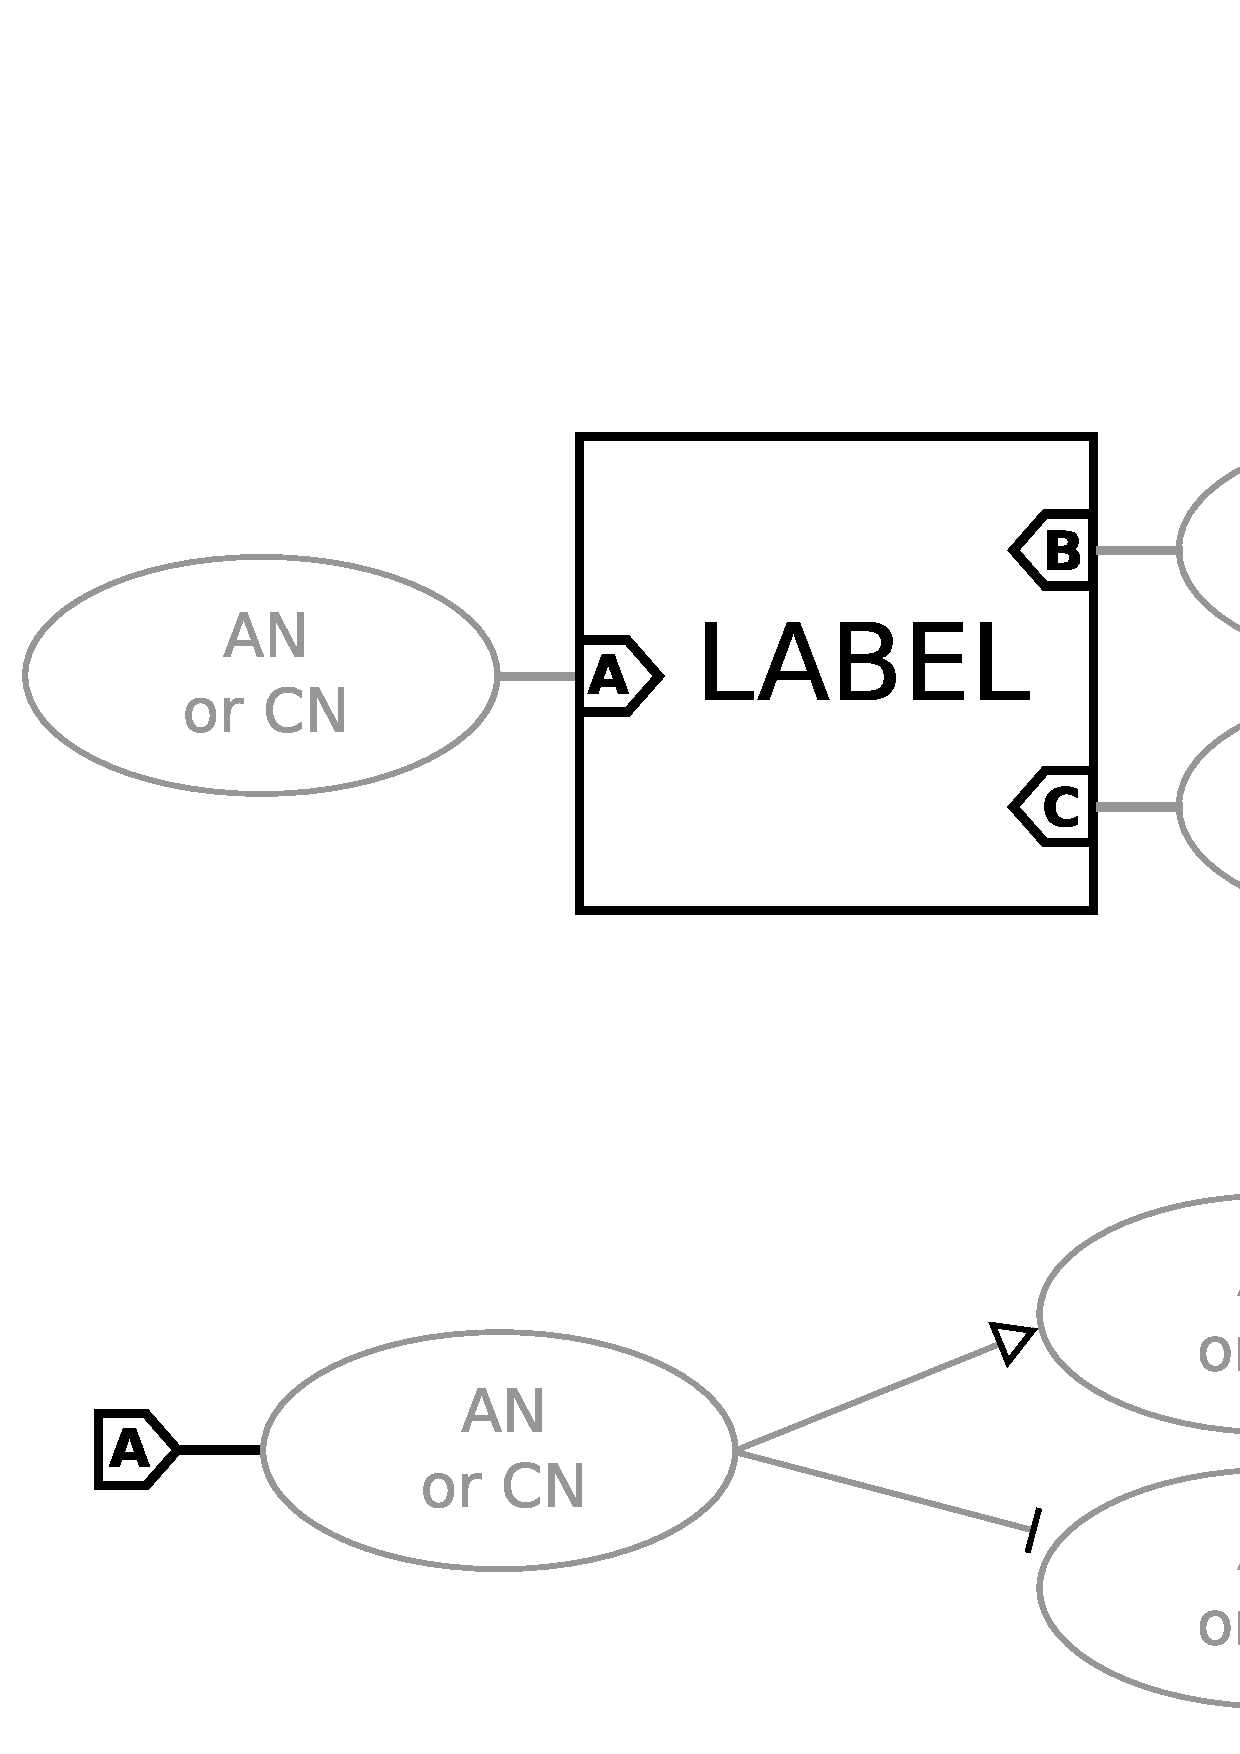
\includegraphics[scale = 0.22]{images/submap}
  \caption{The \AF glyph for \glyph{submap}. (Upper part) folded submap. (Lower part) content of the submap.}
  \label{fig:submap}
\end{figure}

\fig{submap-folded} represents a \glyph{submap} of inhibitory G-protein coupled receptor signaling. The \glyph{submap} carries five terminals, three linked to biological ANs, and two linked to \glyph{compartments}.  Note that the terminals do not define a ``direction'', such as input or output.  The flux of the activities is determined by the context.

\begin{figure}[H]
  \centering
  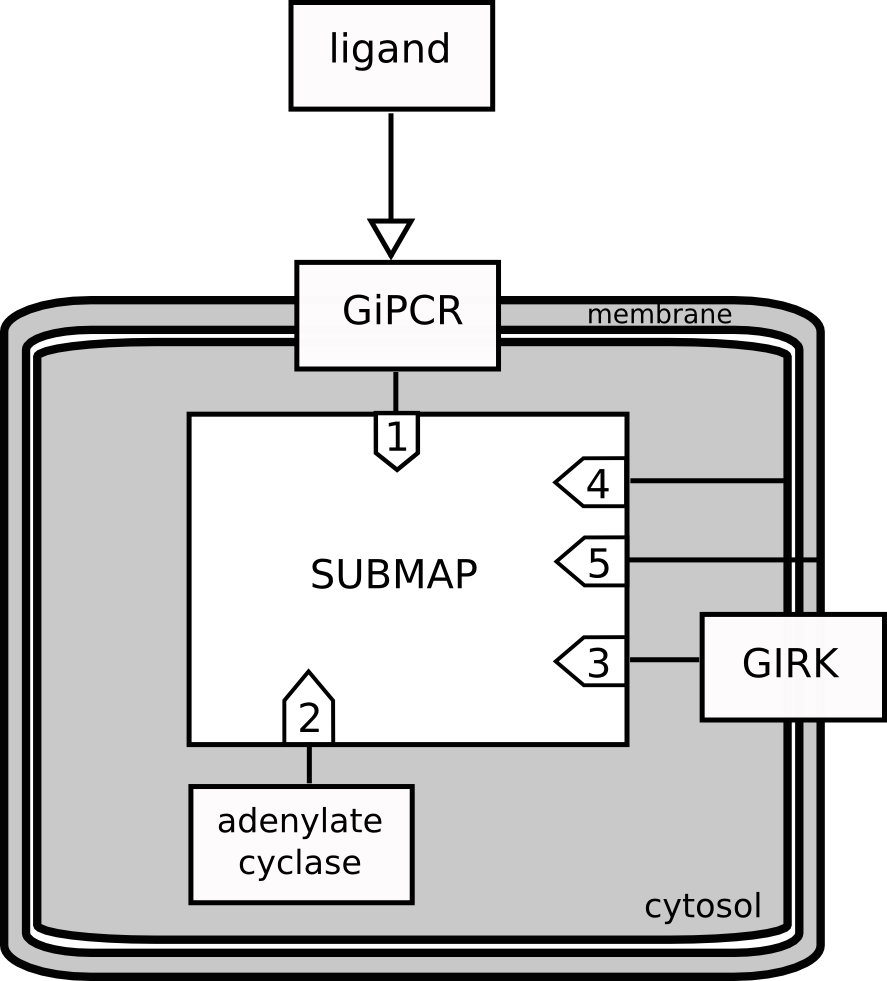
\includegraphics[scale = 0.5]{examples/submap-folded}
  \caption{Example of a submap with contents elided.}
  \label{fig:submap-folded}
\end{figure}

The diagram in \fig{submap-unfolded} represents an unfolded version of a submap.  Here, anything outside the submap has disappeared (e.g., ligand in \fig{submap-folded}), and the internal \glyph{tags} are not linked to the corresponding external \glyph{terminals}.

\begin{figure}[H]
  \centering
  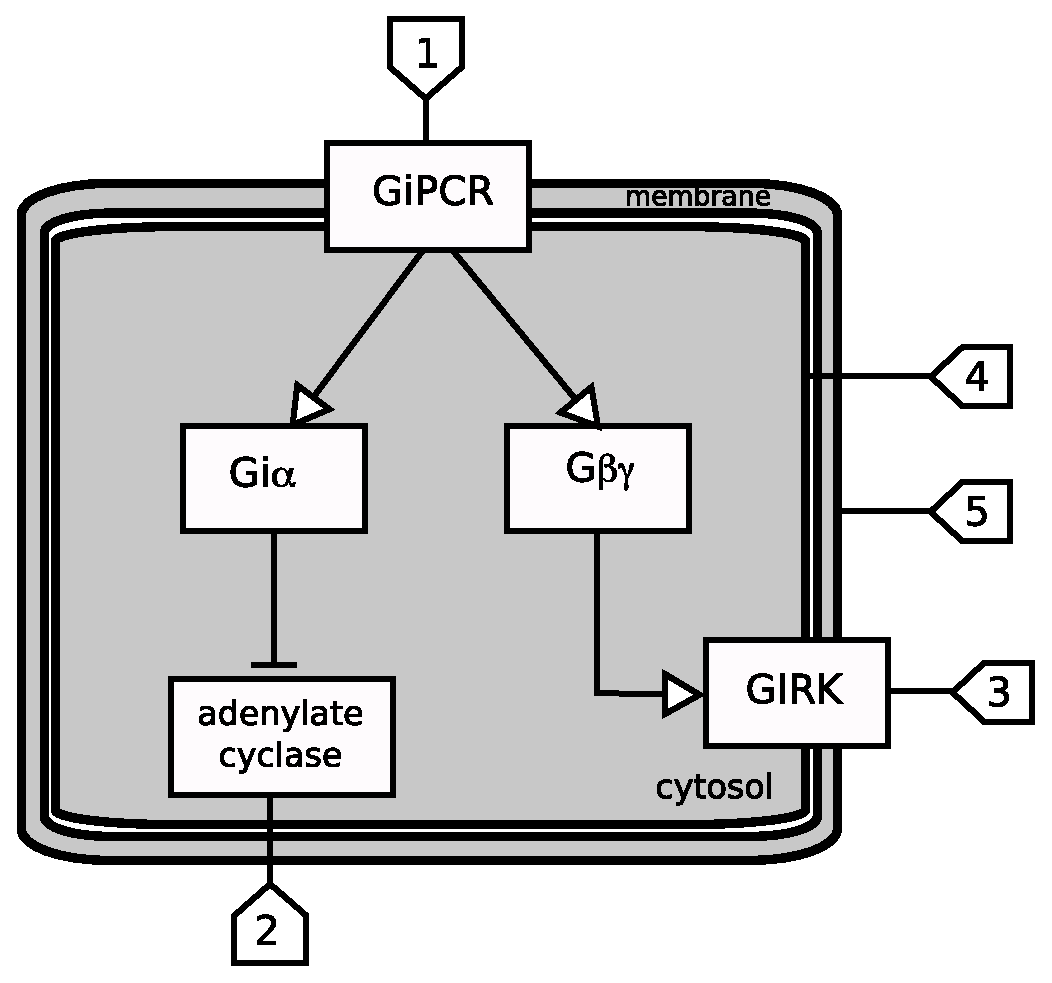
\includegraphics[scale = 0.5]{examples/submap-dissociated}
  \caption{Example of an unfolded submap. The unfolded submap corresponds to the folded submap of \fig{submap-folded}.}
  \label{fig:submap-unfolded}
\end{figure}


%%%%%%%%%%%%%%%%%%%%%%%%%%%%%%%%%%%%%%%%%%%%%%%%%%%%%%%%%%%%%%%%%%%%%%
%%%%                  Arcs
%%%%%%%%%%%%%%%%%%%%%%%%%%%%%%%%%%%%%%%%%%%%%%%%%%%%%%%%%%%%%%%%%%%%%%

\section{Modulation arcs}\label{sec:af:arcs}

Modulation arcs are lines that link ANs together.  The symbols attached to their end extremities indicate their semantics.  The modulation arcs can be used to represent direct influence from one activity to another, such as nicotine to nicotinic acetylecholine receptor activity, or indirect influence.

\subsection{Glyph: \glyph{Positive influence}}
\label{sec:af:positive_infl}

In \SBGNAFLone, a \emph{positive influence} is defined as an action that produces positive or activating effect from one activity to another.   

\begin{glyphDescription}

\glyphSboTerm SBO:

 \glyphOrigin Any \glyph{Activity node} (\sect{af:ANs}) or any \glyph{logical operator} (\sect{af:logic}).
 \glyphTarget Any \glyph{Activity node} (\sect{af:ANs}).
 \glyphEndPoint The target extremity of a \glyph{positive influence} carries an open arrow pointing to the target activity node (\fig{af:positiveInfl}).


\end{glyphDescription}

\begin{figure}[H]
  \centering
  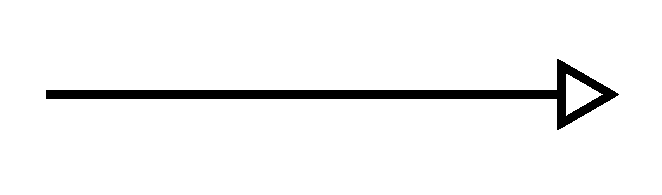
\includegraphics[width = 2in]{images/positiveInfluence}
  \caption{The \AF glyph for \glyph{positive influence}.}
  \label{fig:af:positiveInfl}
\end{figure}

\subsection{Glyph: \glyph{Negative influence}}
\label{sec:af:negative_infl}

A \emph{negative influence} is defined as an action that produces a negative or inhibiting effect from one activity to another.

\begin{glyphDescription}

\glyphSboTerm SBO:0000169 ! inhibition

 \glyphOrigin Any \glyph{Activity node} (\sect{af:ANs}) or any \glyph{logical operator} (\sect{af:logic}).
 \glyphTarget Any \glyph{Activity node} (\sect{af:ANs}).
 \glyphEndPoint The target extremity of a \glyph{negative influence} carries a bar perpendicular to the arc (\fig{af:negativeInfl}).


\end{glyphDescription}

\begin{figure}[H]
  \centering
  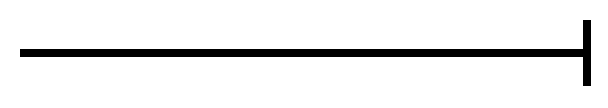
\includegraphics[width = 2in]{images/negativeInfluence}
  \caption{The \AF glyph for \glyph{negative influence}.}
  \label{fig:af:negativeInfl}
\end{figure}



\begin{figure}[H]
  \centering
  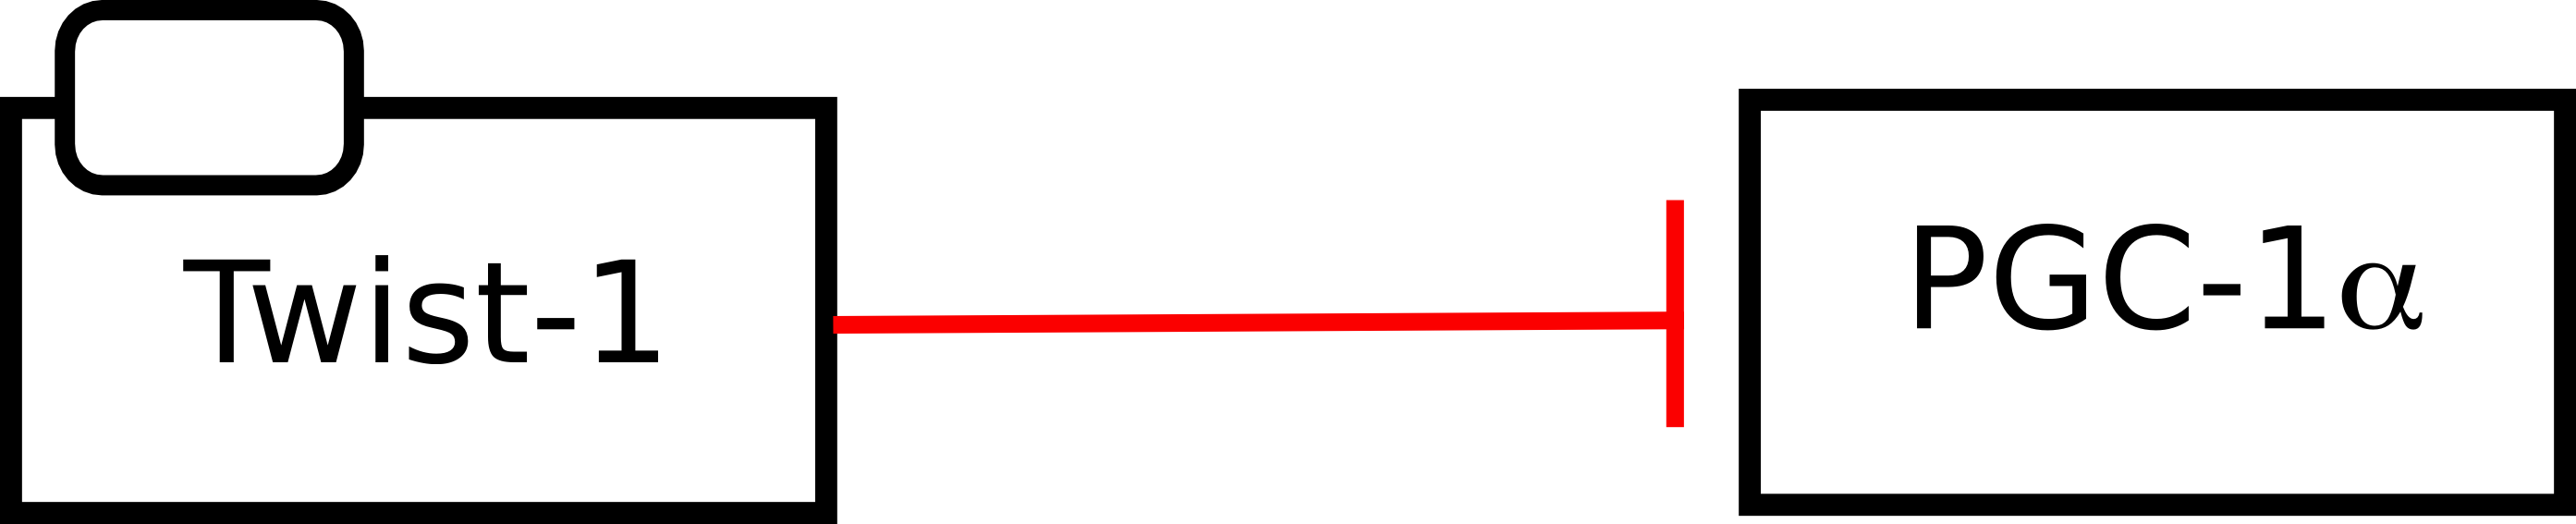
\includegraphics[width = 5in]{examples/ex-negativeInfluence}
  \caption{An example of \glyph{negative influence} from \glyph{"Twist-1"} activity to \glyph{"PGC-1$\alpha$"} activity.}
  \label{fig:af:ex-NI}
\end{figure}
\subsection{Glyph: \glyph{Unknown influence}}
\label{sec:af:unknown_infl}

An \emph{unknown influence} is used when the effect exerted from one activity to another is not well understood. 

\begin{glyphDescription}

\glyphSboTerm SBO:

 \glyphOrigin Any \glyph{Activity node} (\sect{af:ANs}) or any \glyph{logical operator} (\sect{af:logic}).
 \glyphTarget Any \glyph{Activity node} (\sect{af:ANs}).
 \glyphEndPoint The target extremity of a \glyph{unknown influence} carries an open diamond (\fig{af:unknownInfl}).


\end{glyphDescription}

\begin{figure}[H]
  \centering
  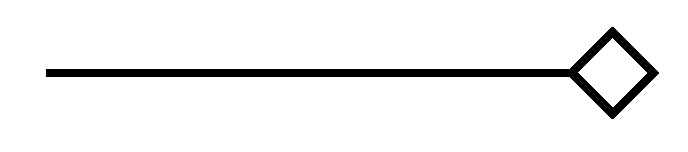
\includegraphics[width = 2in]{images/unknownInfluence}
  \caption{The \AF glyph for \glyph{unknown influence}.}
  \label{fig:af:unknownInfl}
\end{figure}


\subsection{Glyph: \glyph{Necessary stimulation}}
\label{sec:af:trigger}
A \glyph{necessary stimulation} is an influence that has to be present for the target activity to take place (to become true).  An activity modulated by a necessary stimulation can only exist when this stimulation is true, whatever are the other influences this activity is subjected to.

\begin{glyphDescription}

\glyphSboTerm SBO:0000171 ! necessary stimulation

  \glyphOrigin Any \glyph{biological activity} (\sect{af:biologicalActivity}), \glyph{perturbation}  (\sect{af:perturbation}) or any \glyph{logical operator} (\sect{af:logic}).
 \glyphTarget Any \glyph{biological activity} (\sect{af:biologicalActivity}) or \glyph{phenotype} (\sect{af:phenotype}).
 \glyphEndPoint The target extremity of a \glyph{necessary stimulation} carries a perpendicular bar followed by an open arrow pointing to the target activity node (\fig{af:trigger}).  The bar has to be bigger than the based of the arrowhead.

\end{glyphDescription}

\begin{figure}[H]
  \centering
  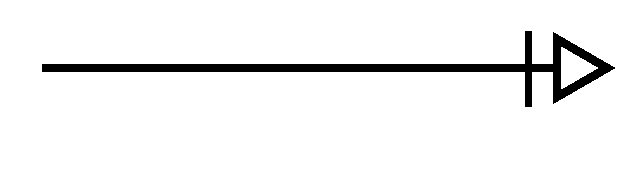
\includegraphics[width = 2in]{images/necessaryStimulation}
  \caption{The \AF glyph for \glyph{necessary stimulation}.}
  \label{fig:af:trigger}
\end{figure}

\begin{figure}[H]
  \centering
  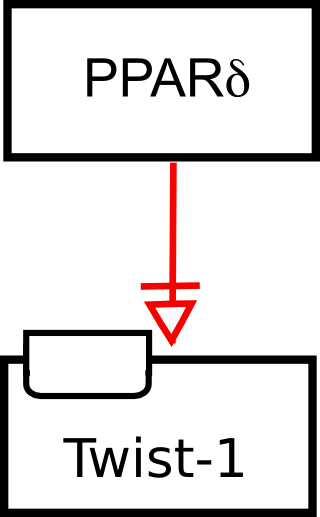
\includegraphics[width = 1.5in]{examples/ex-necessaryStimulation}
  \caption{An example, taken from \fig{af:1}, of \glyph{necessary stimulation} where nuclear hormone receptor \glyph{PPAR $\delta$} transcription factor activity stimulates the gene expression of \glyph{Twist-1}. }
  \label{fig:af:ex-NS}
\end{figure}

%%%%%%%%%%%%%%%%%%%%%%%%%%%%%%%%%%%%%%%%%%%%%%%%%%%%%%%%%%%%%%%%%%%%%%
%%                     Logic arc
%%%%%%%%%%%%%%%%%%%%%%%%%%%%%%%%%%%%%%%%%%%%%%%%%%%%%%%%%%%%%%%%%%%%%%

\subsection{Glyph: \glyph{Logic arc} }\label{sec:af:logicArc}

\glyph{Logic arc} is used to represent the fact that an activity influences the outcome of a logic operator.

\begin{glyphDescription}
 \glyphSboTerm SBO:0000398 ! logical relationship.
 \glyphOrigin Any \glyph{Activity node} (\sect{af:ANs}) or any \glyph{logical operator} (\sect{af:logic}).
 \glyphTarget Any \glyph{logical operator} (\sect{af:logic}).
 \glyphEndPoint No particular symbol is used to represent a logic arc.
 \end{glyphDescription}

\begin{figure}[H]
  \centering
  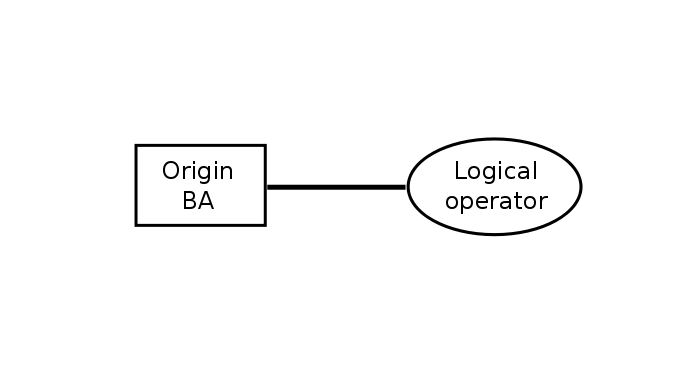
\includegraphics[scale = 0.4]{images/logicArc}
  \caption{The \AF glyph for \glyph{logic arc}.}
  \label{fig:logicArc}
\end{figure}

%%%%%%%%%%%%%%%%%%%%%%%%%%%%%%%%%%%%%%%%%%%%%%%%%%%%%%%%%%%%%%%%%%%%%%
%%                     Equivalence Arc
%%%%%%%%%%%%%%%%%%%%%%%%%%%%%%%%%%%%%%%%%%%%%%%%%%%%%%%%%%%%%%%%%%%%%%

\subsection{Glyph: \glyph{Equivalence arc} }\label{sec:equivalenceArc}

\glyph{Equivalence Arc} is the arc used to represent the fact that all activities or compartments
marked by a \glyph{tag} are equivalent.  Since each AN can only appear once in a compartment, this arc is not going to be used in any main \AFm.  It is useful, however, to show that an AN in a submap and another AN in the main map are equivalent.

\begin{glyphDescription}
 \glyphSboTerm Not applicable.
 \glyphOrigin Any \glyph{Activity node} (\sect{af:ANs}) or any \glyph{compartment}.
 \glyphTarget \glyph{Tag}.
 \glyphEndPoint No particular symbol is used to represent an \glyph{equivalence arc}.
 \end{glyphDescription}

\begin{figure}[H]
  \centering
  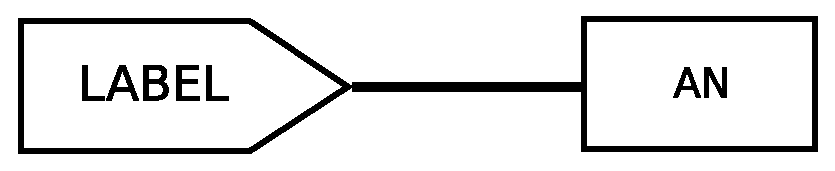
\includegraphics[scale = 0.4]{images/equivalence}
  \caption{The \AF glyph for \glyph{Equivalence arc}.}
  \label{fig:equivalence}
\end{figure}




%%%%%%%%%%%%%%%%%%%%%%%%%%%%%%%%%%%%%%%%%%%%%%%%%%%%%%%%%%%%%%%%%%%%%%
%%%%                   Logical operators
%%%%%%%%%%%%%%%%%%%%%%%%%%%%%%%%%%%%%%%%%%%%%%%%%%%%%%%%%%%%%%%%%%%%%%

\section{Logical operators}\label{sec:af:logic}

\subsection{Glyph: \glyph{And}}
\label{sec:af:and}

The glyph \glyph{and} is used to denote that all the \glyph{AFNs} linked as input are necessary to produce the output.

\begin{glyphDescription}
 \glyphSboTerm SBO:0000173 ! and.
 \glyphOrigin More than one AFN (\sect{af:ANs}) or logical operator (section~\ref{sec:af:logic}).
 \glyphTarget  Modulation arc (\sect{af:arcs}).
 \glyphNode \glyph{And} is represented by a circle carrying the word ``AND''.
\end{glyphDescription}

\begin{figure}[H]
  \centering
  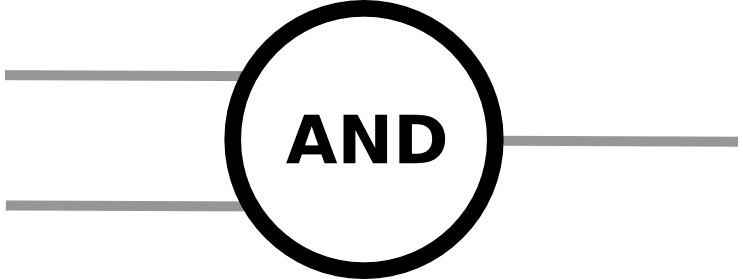
\includegraphics[scale = 0.5]{images/and}
  \caption{The \AF glyph for \glyph{and}. Only two inputs are represented, but more would be allowed.}
  \label{fig:af:and}
\end{figure}

\subsection{Glyph: \glyph{Or}}
\label{sec:af:or}

The glyph \glyph{or} is used to denote that any of the \glyph{ANs} linked as input is sufficient to influence the target activity.

\begin{glyphDescription}
 \glyphSboTerm SBO:0000174 ! or.
 \glyphOrigin More than one \glyph{AN} (\sect{af:ANs}) and \glyph{logical arcs} (section~\ref{sec:af:logicArc}).
 \glyphTarget  \glyph{Modulation arc} (\sect{af:arcs}) other than \glyph{equivalence arc}.
 \glyphNode \glyph{Or} is represented by a circle carrying the word ``OR'', with two connectors located at the opposite side for inputs and output.
 \end{glyphDescription}

\begin{figure}[H]
  \centering
  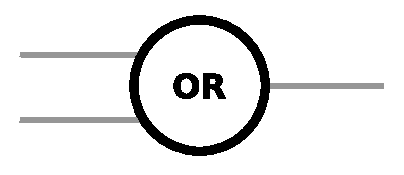
\includegraphics[scale = 0.5]{images/or}
  \caption{The \AF glyph for \glyph{or}. Only two inputs are represented, but more would be allowed.}
  \label{fig:af:or}
\end{figure}


\begin{figure}[H]
  \centering
  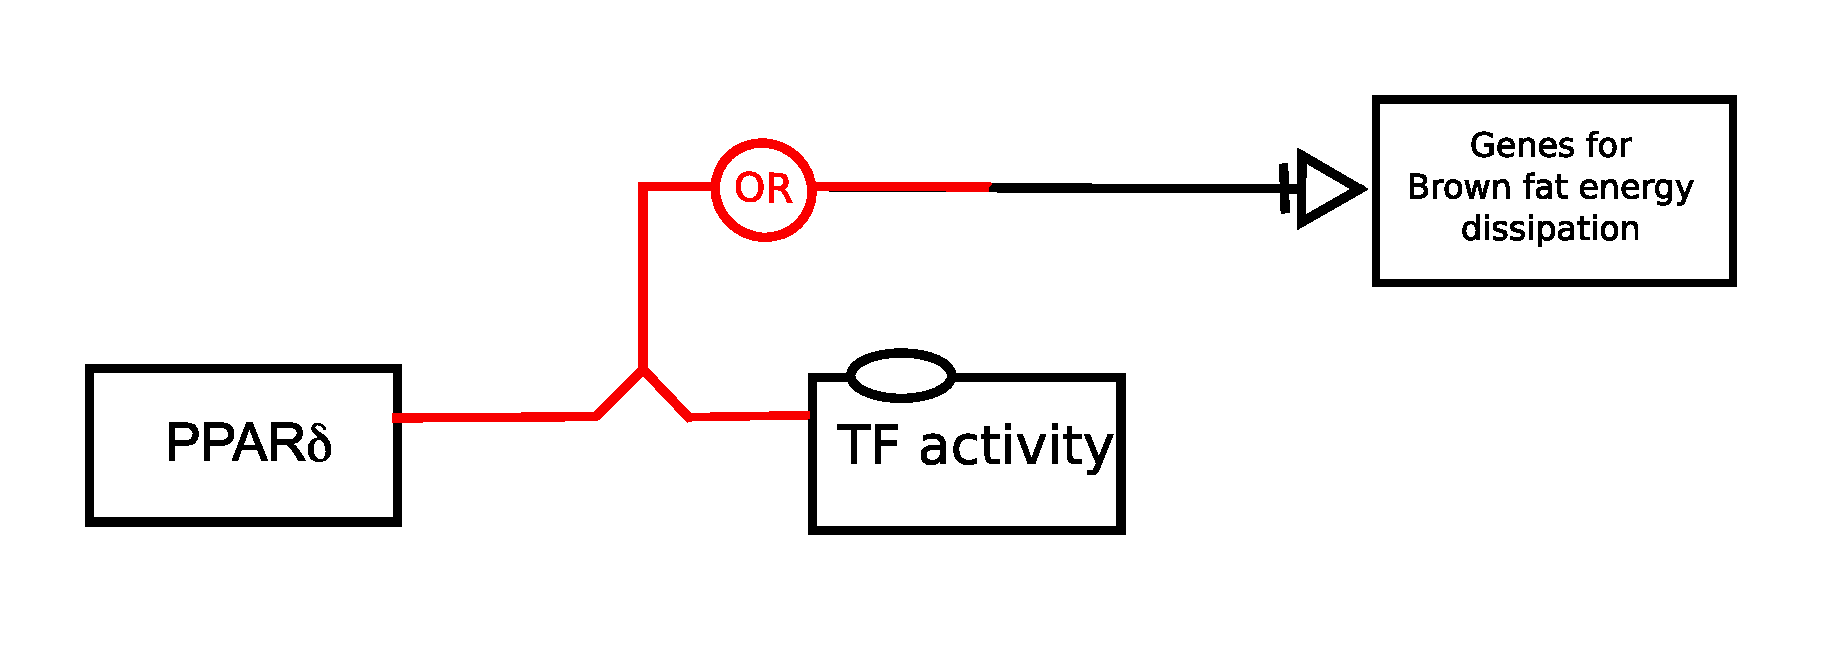
\includegraphics[scale = 0.5]{examples/ex-or}
  \caption{An example of the \glyph{or} logic operator, where the \glyph{"Genes for brown fat energy dissipation"} is stimulated by either the \glyph{PPAR delta} activity or an \glyph{unspecified transcription factor} activity.}
  \label{fig:af:ex-or}
\end{figure}

\subsection{Glyph: \glyph{Not}}
\label{sec:af:not}

The glyph \glyph{not} is used to denote that the \glyph{AN} linked as input cannot produce the output.

\begin{glyphDescription}
 \glyphSboTerm SBO:0000238 ! not.
 \glyphOrigin One AN (section~\ref{sec:af:ANs}) or logical operator (section~\ref{sec:af:logic}).
 \glyphTarget A modulation arc (section~\ref{sec:af:ANs}).
 \glyphNode \glyph{Not} is represented by a circle carrying the word ``NOT''.
 \end{glyphDescription}

\begin{figure}[H]
  \centering
  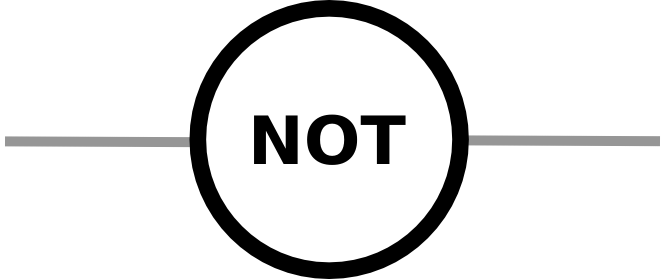
\includegraphics[scale = 0.5]{images/not}
  \caption{The \AF glyph for \glyph{not}.}
  \label{fig:af:not}
\end{figure}

%%%%%%%%%%%%%%%%%%%%%%%%%%%%%%%%%%%%%%%%%%%%%%%%%%%%%%%%%%%%%%%%%%%%%%
%%                     delay
%%%%%%%%%%%%%%%%%%%%%%%%%%%%%%%%%%%%%%%%%%%%%%%%%%%%%%%%%%%%%%%%%%%%%%

\subsection{Glyph: \glyph{delay}}\label{sec:delay}

The glyph \glyph{delay} is used to denote that the \glyph{activity node} linked as input does not produce the influence immediately.

\begin{glyphDescription}
 \glyphSboTerm SBO:0000225 ! delay.
 \glyphOrigin One \glyph{AN} (section~\ref{sec:af:ANs}) or and a \glyph{logical arc} (section~\ref{sec:af:logicArc}).
 \glyphTarget A \glyph{modulation arc} (section~\ref{sec:af:ANs}) other than \glyph{equivalence arc}.
 \glyphContainer \glyph{Delay} is represented by a circle, with two connectors located at the opposite side for inputs and output.
 \glyphLabel \glyph{Delay} is identified by the greek letter ``$\tau$`` (``TAU'') placed in an unbordered box attached to the center of the node.
 \glyphAux \glyph{Delay} does not carry any auxiliary items.
\end{glyphDescription}

\begin{figure}[H]
  \centering
  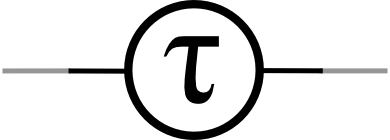
\includegraphics[scale = 0.5]{images/delay}
  \caption{The \AF glyph for \glyph{delay}.}
  \label{fig:delay}
\end{figure}
\normalcolor
 